%! Tex program = xelatex
\documentclass[UTF8]{article}
\usepackage{indentfirst}
\usepackage{graphicx} 
\usepackage{amsmath}  
\usepackage{float}   
\usepackage{listings}

\title{Discrete Mathematics}
\author{Zhengren Wang 2019081308021}
\date{06/02/2020 Tue}
\begin{document}
\maketitle 

\part{10.3}
\begin{description}
    \item[15]Represent the given graph using an adjacency matrix. \\
        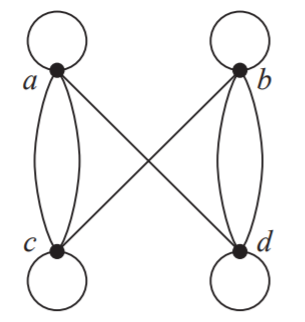
\includegraphics[scale=0.3]{../imgs/10_3_15.png}



    \item[39]Determine whether the given pair of graphs is isomorphic. Exhibit an isomorphism or provide a rigorous argument that none exists  \\
        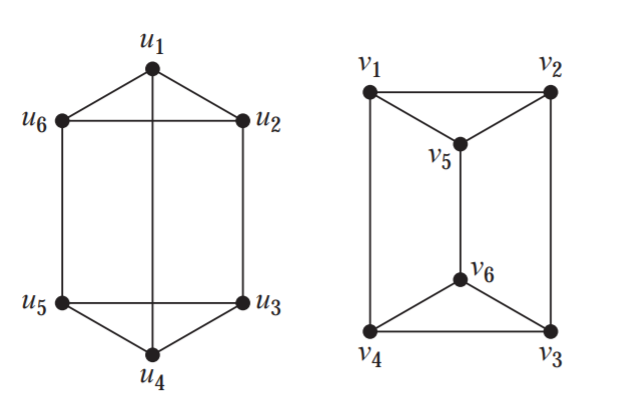
\includegraphics[scale=0.3]{../imgs/10_3_39.png}


    \item[45]Show that isomorphism of simple graphs is an equivalence relation. \\

\end{description}

\end{document}
